\documentclass{article}
\usepackage[english]{babel}
\usepackage[a4paper,top=2cm,bottom=2cm,left=2.5cm,right=2.5cm,marginparwidth=1.75cm]{geometry} 
\usepackage{hyperref}
\usepackage[authoryear]{natbib}
\usepackage{graphicx}
\usepackage{fancyhdr}

% CUSTOM PACKAGE
\usepackage{booktabs}
\usepackage{tabularx}
\usepackage{color, colortbl}
\definecolor{anti-flashwhite}{rgb}{0.95, 0.95, 0.96}
\usepackage{float}

\bibliographystyle{rusnat}

\pagestyle{fancy}
\fancyhf{}
\lhead{Szymon Gałecki, Frederik Bechmann \& Ellen Daetz}
\rhead{Project Name}
\rfoot{Page \thepage}

\title{Geospatial Aspects of Copenhagen's Rental Market}
\author{Szymon Gałecki, Frederik Bechmann \& Ellen Daetz}
\date{26-05-2023}

\begin{document}

\maketitle

\begin{figure}[!htbp]
    \centering
    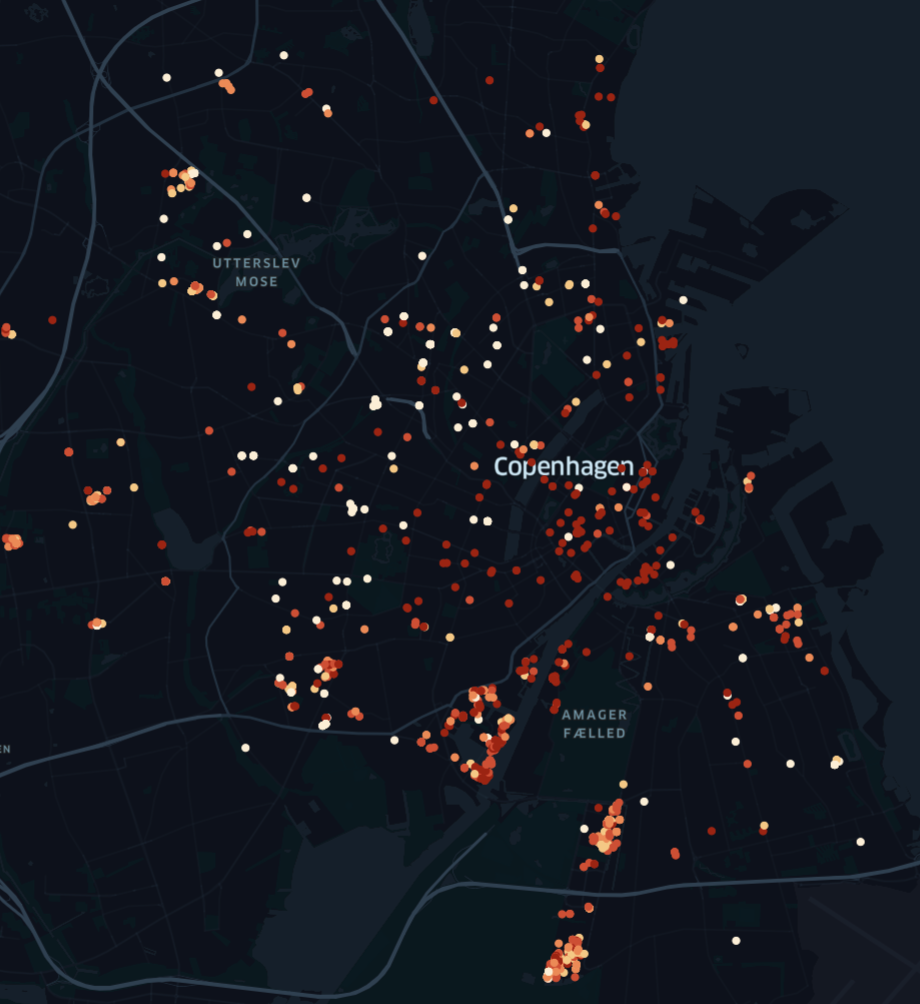
\includegraphics[scale=0.5]{images/front_page.png}
\end{figure}

\newpage

\section{Introduction}
%Here you provide the context and motivation for the problem. What are your research questions, or what does your prototype intend to do/solve? Explain the particular spatial problem you are tackling and its relevance. 


%and the rental market can be hard to navigate in. You might find a rental at one out of many websites for rentals or know someone who rents out a place.  Furthermore you often have to compromise with location and price. In general we do not have a lot of knowledge about the rental market.\\ 

Today, many people have to rent a place to live in Copenhagen because it is too expensive to buy an apartment or because they are only looking for a temporary home. Young people are moving to the city to study while others have to work. Our personal experience is that finding a place to live in Copenhagen can be challenging. Ejendeom Danmark confirms that looking over the last year the number of available rentals have decreased with 0.8 percentage points\footnote{https://ejd.dk/nyheder/lejemarkedet-fortsat-praeget-af-boligmangel}. Furthermore Berlingske writes that the increasing demand means that the prices have increased with 2.6\% across the country. And in Copenhagen there are now equally many rentals as private apartments\footnote{https://www.berlingske.dk/samfund/buldrende-priser-paa-lejeboliger-faar-flere-partier-til-at-raabe-op-i}. Despite of this we do not know a lot about the rental market and are probably often compromising with location, price and size among others.\\
\\ 
The purpose of this paper is therefore to give insights in the rental market in Copenhagen. Focus will be on price variation in relation to spatial location and spatial distances. The questions of interest are written below. \\
\\
\centerline{What influences the rental prices in Copenhagen? (linear regression and Moran's I)}
\centerline{Can we obtain a continuous map of rent prices from discrete observations? (Interpolation)} 

\subsection{Background}
%Provide context (historical, cultural, technical) for your project and introduce the background and related work in literature (cite or list relevant literature on the research problem; list other scripts and software in this area etc.) Give an overview of the (cultural, historical, social, technical, etc.) problems to be solved by the project and the role of the different digital tools in achieving the aims of the project Specify your approach and why you have chosen it.

There is not a lot of related work in literature writing about the rental market in Copenhagen. 
However Landsbyggefonden writes an overall report on rent in Denmark every year in which they analyse the rent in regions and municipalities on different types of properties. The report clearly shows that the rent is higher in Copenhagen and that rent is increasing these years. Moreover it is clear that size and location has an impact on the rent \footnote{https://lbf.dk/media/1557414/huslejestatistik-2020.pdf}.\\
\\
Furthermore we know that location has the greatest impact on prices related to the housing market. Buyers often have concerns in regards to ocean view, green areas, school areas, popularity of the area, and transport time to the job\footnote{https://www.bolius.dk/saadan-fastsaettes-prisen-paa-ejerboliger-17798}. This paper will therefore look more detailed into clustering and distance to nearest metro. 

\subsection{Distance to metro}
One assumption we want to research is if prices are influenced by the distance to the nearest metro station. To research the assumption we will make a linear regression \ref{Linear Regression Method} between the distance to the nearest metro station and the normalized rental price. The distance to the metro will be based on Open Street Map data that provides us with metro station coordinates. To find the distance, we compute the distance between two geographic coordinates containing longitude and latitude. The formula used for calculating the distances is called Haversine \ref{haversine}. 

\section{Data acquisition}
%List and cite all sources of data used in this paper, comment on their fitness for purpose (format, quality, and provenance). Focus on the spatial component of your data, its origin, and precision and reliability. 

The two primary sources are Boligsiden.dk and Boligzonen.dk. None of these sources contains data on all rentals in Copenhagen. There are many more websites where a rentee may look for apartments to rent including BoligPortal, Heimstaden, Facebook, DBA among others. In this project around two thousand records in each data set is collected which is enough for looking at the overall trends. 

\subsection{Boligsiden data}
The data is extracted from Boligsiden's database as a .xlsx file. The file contains all rentals at boligsiden.dk in the time period from April 2022 to April 2023. Boligsiden.dk collaborates with all the real estate agents in Denmark and are leading on the real estate market but they also receive information on rental properties. Thus each row in the data set represents a rental reported by a danish real estate agent with information about the property and real estate agent. Overall rental information includes property details, rental prices, location, real estate details, status and visibility on the website. In this project we will use the location given as geographic coordinates to map the apartments. Investigating the data we discovered that most of the rentals if not all are project apartments meaning they are often new buildings with a high rent. 

\subsection{Boligzonen data}
This data set contains scraped data from boligzonen.dk. The data is scraped by running our own script build in Go on a given day and is then saved to a .csv file. This means that information in this data set is restricted by the data shown on their website. The main difference between Boligsiden and Boligzonen data is the time frame. While Boligsiden captures data over a year, Boligzonen data is a snapshot of the apartments available in Copenhagen on a given day. For each apartment we gathered information about the number of rooms, square meter area, rent price, price per square meter, geographic coordinates and normalized rent. By looking at the website it is clear that the apartments are mainly rented out by private people. 

\subsection{Combining the data sets}
This project seeks insights in the rental market of Copenhagen. The initial idea was to collect data from different sources and then combine it into one single data set which could be used for the analysis. Since we ended up with data from only two sources and because the data sets differ mainly in the type of rentals and the time frame, we decided to keep the data sets separated when doing the analysis. The apartments from each source and their prices are visualised figure 1 through a density plot. Notice that the orange grading tells that there are more expensive apartments with a square meter price higher than 200 Danish Crowns per month at Boligsiden. The apartments are mapped on figure 2. The figure shows how rental apartments at Boligzonen are more spread out than at Boligsiden because Boligsiden mainly contains project apartment that are build in specific areas. In conclusion we have decided to analyse both the data sets and then compare the results to see if there are some interesting differences. 

\begin{figure}
    \centering
    \begin{minipage}{0.4\textwidth}
        \centering
        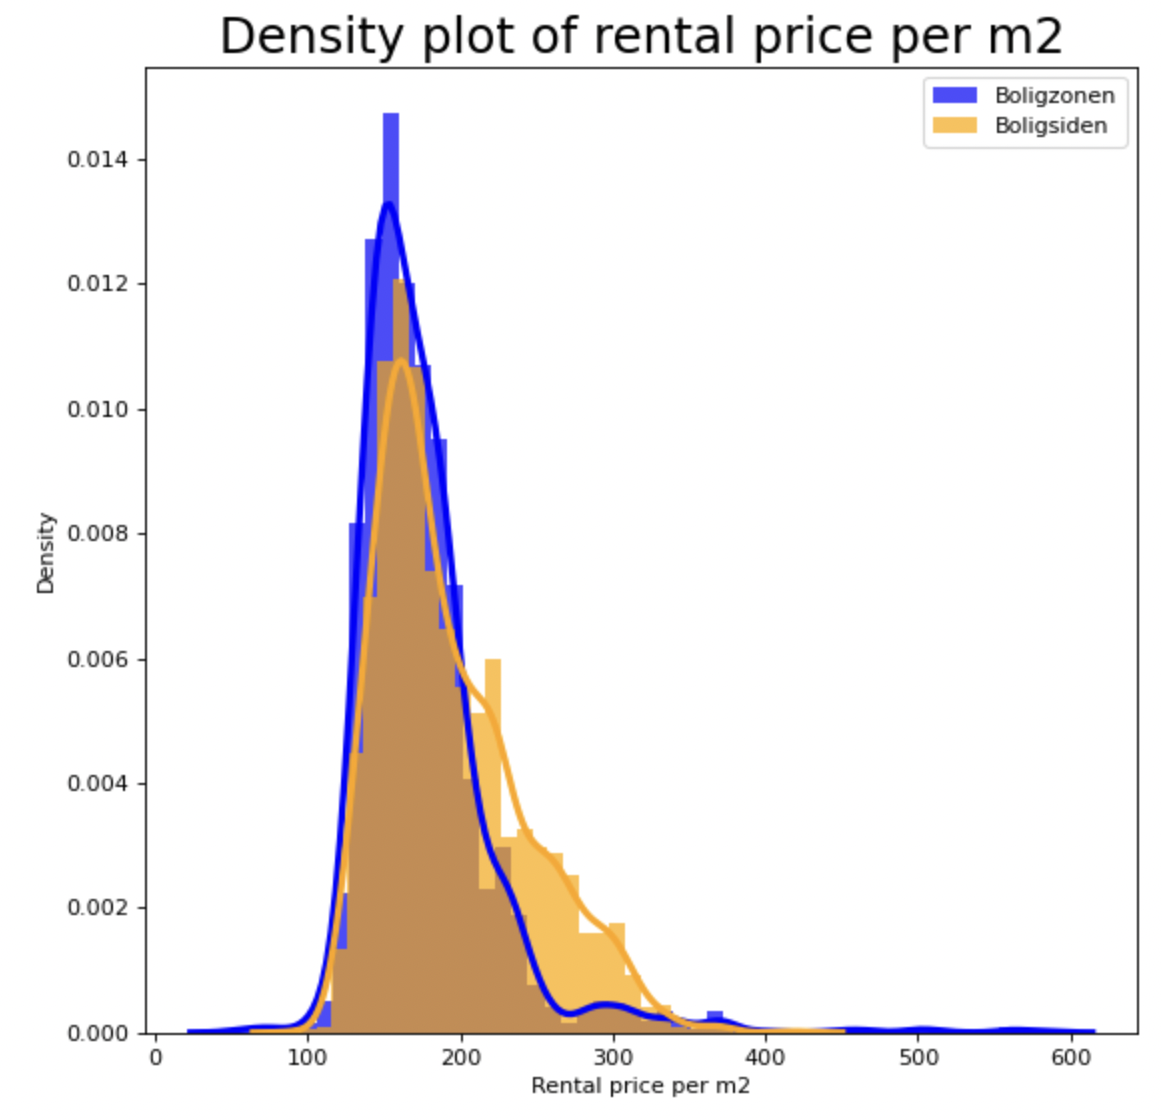
\includegraphics[width=1\textwidth]{images/DensityPlot.png} % first figure itself
        \caption{Density plot of rental price per square meter}
    \end{minipage}\hfill
    \begin{minipage}{0.6\textwidth}
        \centering
        \includegraphics[width=1\textwidth]{images/apartments.png} % second figure itself
        \caption{Boligsiden and Boligzonen apartments}
    \end{minipage}
\end{figure}

% \begin{figure}[H]
%     \centering
%     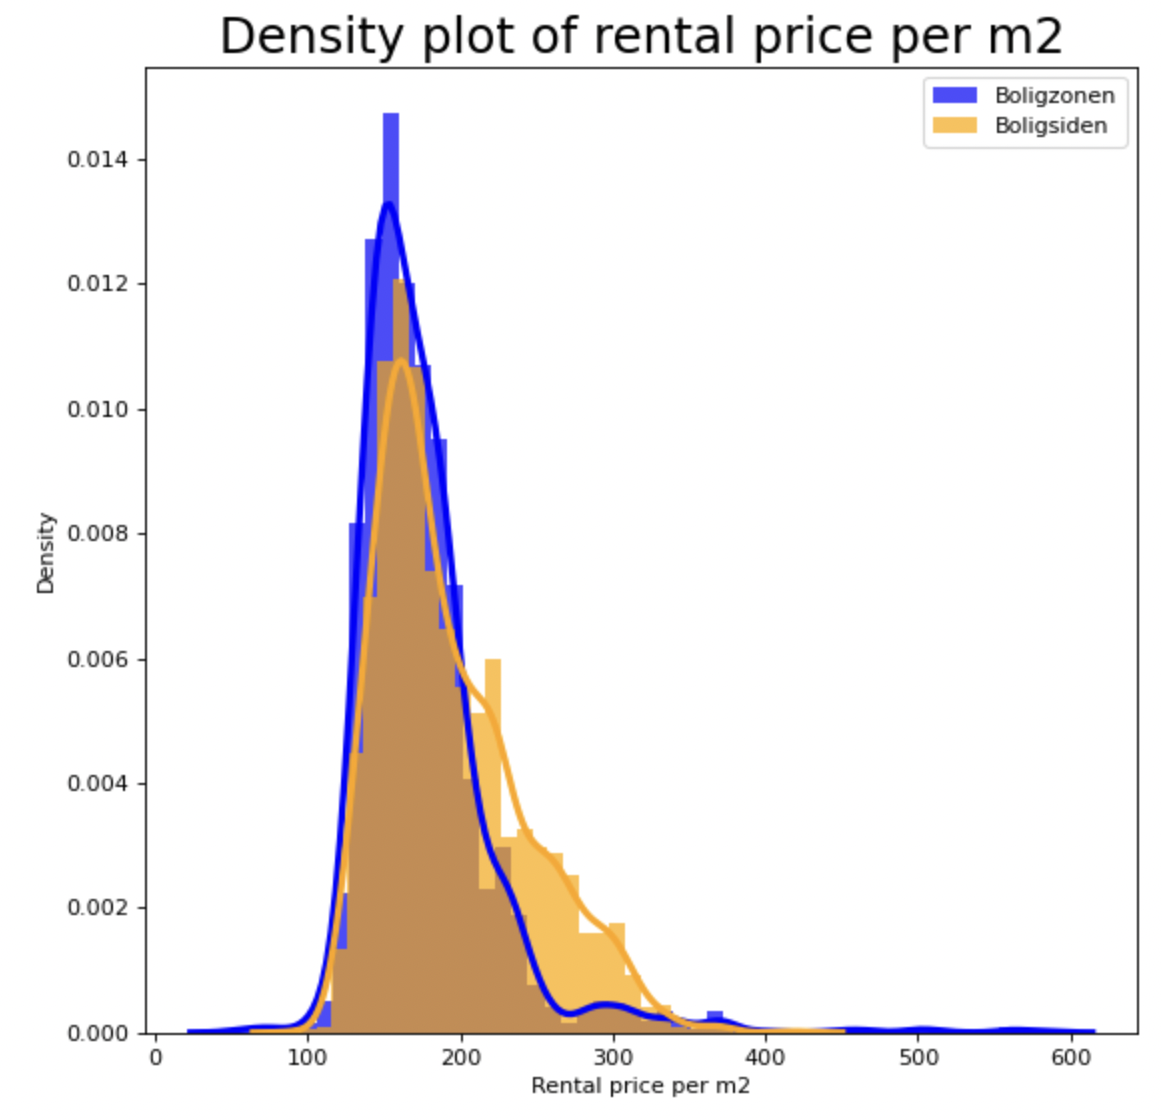
\includegraphics[width=0.5\textwidth]{images/DensityPlot.png}
%     \caption{Density plot of rental price per square meter}
% \end{figure}

% \begin{figure}[H]
%     \centering
%     \includegraphics[width=0.7\textwidth]{images/apartments.png}
%     \caption{Boligsiden and Boligzonen apartments}
% \end{figure}

\section{Data processing}
%Provide details of data manipulation and transformation. Name challenges, if any. Link to processing scripts where relevant.

\subsection{Boligsiden.dk}
As mentioned earlier Boligsiden data set contains a lot of irrelevant information that needs to be filtered out before analysing. Our goal is to only keep columns that are in the Boligzonen data set so that we have similar data sets. Furthermore we like to rename the columns so that they have the same names. This reduces the risk of misunderstandings. For example we found that the column called "per\_area\_price" did not contain price divided by area which was represented in the other data set. Thus we had to add a column with the square meter price. Boligsiden columns are id, available\_from, rooms, area, rent, norm\_rent, longitude and latitude. We also removed duplicates. An apartment might appear in more than one row if it has been put on the market multiple times. These duplicates are interesting because they look like there were many rental apartments in a specific area when in reality it is the same apartment, hence we decided to only keep the latest rental information for each apartment. To remove duplicates we grouped on address, sorted by created\_at and kept the latest. 

\subsection{Scrape on 1.04.2023 from boligzonen.dk}
Data scraped from boligzonen gave good first impression. The number of records matched exactly the number of properties listed in Copenhagen on boligzonen.dk. Only 6 properties out of 1886 didn't have geographical coordinates. There was nice linear dependency between the price and area, properties were clustered by number of rooms. There was just a single problem, we had 434 duplicates or near duplicates out of 1886 properties. First approach was to check a single case at random. We picked a 38 square meter property at Øresundsvej, listed for 9300 DKK. At boligzonen.dk we found 3 offers with the same values in the fields that we scraped for each apartment. We can't know if these are 3 different listing for 3 different apartments but we have to make assumption that they are, as long as they have different case numbers. That is why we have to modify the scraping script to include a new field that will serve as an external unique id for each property, and redo the scraping process.
\begin{figure}[!htbp]
    \centering
    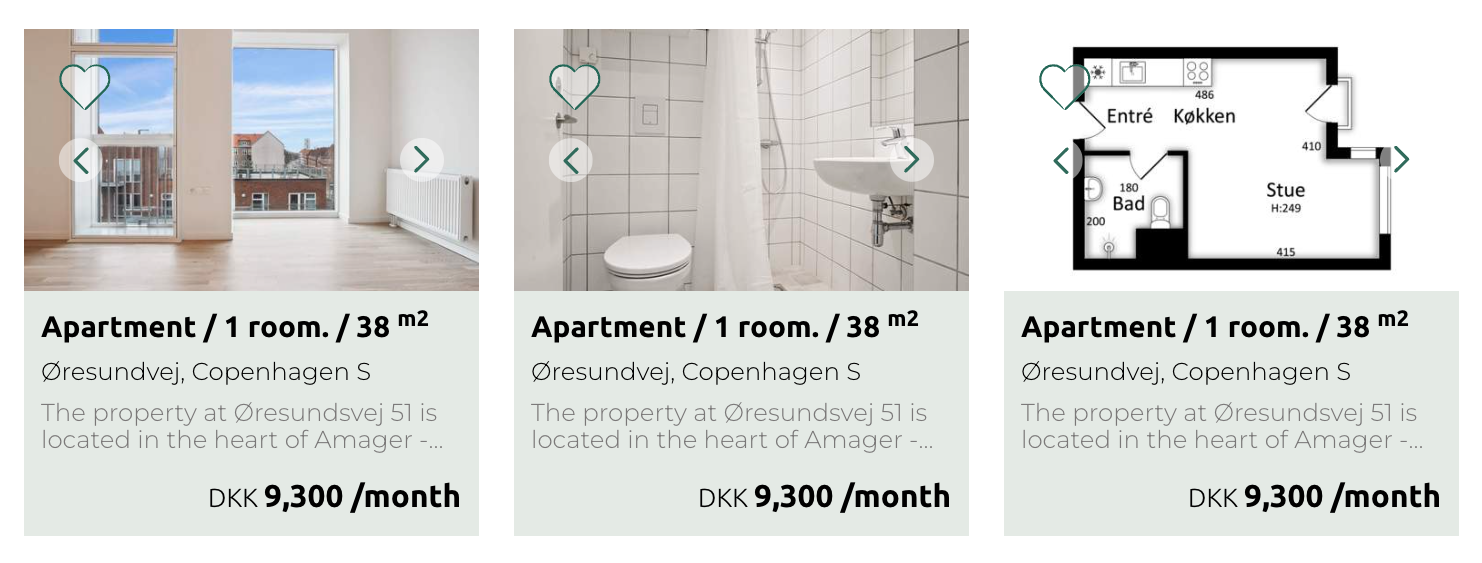
\includegraphics[scale=0.3]{images/duplicates.png}
    \caption{Apartments that seemed to be a duplicate of a single apartment}
    \label{fig:my_label}
\end{figure}

\subsection{Scrape on 17.04.2023 and 20.04.2023 from boligzonen.dk}
Case number that serves as unique id for each property showed that we actually get a lot of duplicates when scraping. We observed that the number of duplicates is connected to scraping duration. Originally we used Python for scraping but it took at least 15 minutes and sometimes even 30. On average it resulted in more than 10\% of duplication. We built another scraper in Go that operated concurrently and took around 4 minutes to go through 2000 pages. While it was significantly faster, it's duplication rate didn't stabilise at concrete value but ranged from 1\% to 20\%. Changes applied on the website during scraping were the most probable reason for the duplication rate fluctuation. To obtain dataset with lower duplication rate we scraped the website 3 times, combined the results and got rid of duplicates. Resulting dataset has duplication rate of 0.1\% which translates to losing 2 records out of 2000.

\section{Method}

\subsection{Linear Regression} \label{Linear Regression Method}
Linear regression can explain the relation between two variable and how one variable depend the other. Thus, we look into how the distance to the nearest metro impact the normalized rental price. It is not given that the relation between two variables is linear. To explore if the variables can be described by a linear regression we computed the R-squared value. The R-squared value is the percentage of the dependent variable variation that a linear model explains. The question is then when to accept the R-squared value? This depends on the scenario and purpose. If the purpose is to predict something the R-squared value is more important. Meanwhile if the purpose is to describe a relationship overall it is not as important\footnote{https://www.statology.org/good-r-squared-value/}. Furthermore we computed the coefficient to examine if there is a positive or negative correlation. 

%Lastly the p value is used to describe if there is a correlation\footnote{https://statisticsbyjim.com/regression/interpret-coefficients-p-values-regression/}. 

\subsection{Haversine} \label{haversine}
There are multiple ways to compute a distance between two points. The easiest way is to use Pythagoras equivalence to calculate the Euclidean Distance. The Euclidean distance describes the distance between two points on a flat surface. Since the earth is not flat but a sphere a more precise distance would be calculated using the Haversine formula to find the great circle distance \cite{Lecture10}. Furthermore both methods compute the straight line distance and not the Manhattan distance for the distance walking on the streets. This might give some uncertainty because the distance does not represent the actual travel time from a rental apartment to the metro if for example the straight line distance is through a building where you cannot pass through. 

\subsection{Spatial weights}
As a means to represent the spatial structure in our data we compute a spatial weight matrix. We initially computed block weights where each apartment was in neighbourhood with other apartments in the same city areas. However, the inductive bias imposed by the arbitrary city area borders did not seem like a good fit for autocorrelation of rent pricing. In the literature of a closely related problem; spatial dependence of property pricing, \cite{ozyurt} uses binary k-nearest neighbour with values 5, 8 and 10 of \textit{k}, while \cite{hyun}, in spatial dependence of apartment transaction prices, uses the inverse distance function with a critical distance band. 

Inspired by the above, we opted for kernel spatial weights with a Gaussian function that weighs closer apartments exponentially higher, as this abides by Tobler's first law (that "everything is related to everything else, but near things are more related than distant things."). Every apartment outside a distance band of a given apartment was considered non-neighbour, i.e. 0 weight. To accommodate for the fact that there was a large difference in density across areas of our data we chose an adaptive distance band for each point by using the \textit{k}th-nearest neighbour as the cut-off. We chose to test \textit{k}-values of 2, 6, 8 and 10 as this allowed us to compute the spatial autocorrelation for different neighbourhood sizes: From apartment blocks to smaller city areas. Apartments were added a small and insignificant Gaussian noise to the latitude and longitude to avoid location duplicates as these resulted in errors in the computation.

% TODO: Consider block weights for Frederiksberg vs Copenhagen

\subsection{Moran's I \& spatial autocorrelation}

We compute Global Moran's I, which measures the general clustering of the data. In other words, it measures if nearby points are similar in terms of the variable(s) of interest, here rent price. To increase the robustness of the study, Moran's I is computed for 999 random permutations in a Monte Carlo simulation. The result is an assessment of the likelihood of obtaining a similar Moran's I as our data given random data (i.e. no autocorrelation). If we find that the result is unlikely to happen by chance then we can be more confident in the result, and vice versa. 

\subsection{Inverse distance weighted interpolation}
This method works on the assumption that objects that are close to each other are similar. It is used to predict the value for point with location, given points with known location and value. Interpolated value is constructed out of known values scaled by the inverse distance to the interpolated point. This means that points that are closer to the interpolated point will have a greater influence on the constructed value than points that are further away. To weaken the influence of points that are far away we can increase the power parameter. Value of power parameter has to be tuned for source data but for geo-spatial applications it is usually set to 1 or 2.

K-nearest neighbors algorithm is used to determine the set of known values for an interpolated value. It is relatively safe to use as there is almost no negative consequence on choosing number of neighbors that is too big. If we have many neighbors in close proximity, we obtain an interpolated value with high confidence. If we have many neighbours that are far away from interpolated point, their influence on interpolated value is minimal.

Points for which values of rent are interpolated are formed into a square grid that covers the area of Copenhagen. By tuning the density of that grid we modify the resolution of our interpolation. The value of k-nearest neighbours is tuned for the grid density, so that majority of apartments are used for interpolation. 

The result is a continuous map of rent prices in Copenhagen with outlined city areas.




\section{Results}

\subsection{Boligzonen}

The results of \textbf{Moran's I} on the Boligzonen data are provided in table \ref{morans_I} for each choice of \textit{k}-nearest neighbour in the spatial weights. For all \textit{k}-values we see a significant pseudo p-value, i.e. below the standard 0.05, and we can for each case reject the null hypothesis. Appendix A shows the Monte Carlo distributions of randomized data compared to the Moran's I values. As we have done multiple hypothesis tests (4), we may correct the p-value threshold with Bonferroni Correction: $threshold = \frac{\alpha}{n} = \frac{0.05}{4} = 0.0125$. As such, all the tests still pass significance. Furthermore, since the Moran's I value is positive in each case, we can say that apartments with high and/or low rent are spatially clustered more than we would randomly expect. This is clearest when \textit{k} equals \textit{2}.

\begin{table}[H]
\renewcommand{\arraystretch}{1.3}
\label{morans_I}
\centering
\begin{tabular}{|c|c|c|c|}
\hline
\bfseries \textit{k-value} & \bfseries Moran's I & \bfseries pseudo p-value\\
\hline\hline
2 & 0.74 & 0.01 \\
6 & 0.55 & 0.01 \\
8 & 0.5 & 0.01 \\
10 & 0.47 & 0.01 \\
\hline
\end{tabular}
\caption{Moran's I results for different values of \textit{k}-nearest neighbor in adaptive kernel spatial weights on the Boligzonen data.}
\end{table}



The results of \textbf{metro distance and rental price correlation} on Boligzonen data are provided in figure \ref{fig:dist_boligzonen}. Overall the figure shows that most apartments are within a thousands meter to the nearest metro and that the normalized rental price for these apartments vary a lot. At the same time most apartments further away from a metro station have a normalized rent up to around 200 crowns. Performing the linear regression method we get the result of the R-squared value to be 0.048 and the result of the coefficient to be -0.0066. In other words 4,8\% of the variance in the rental price can be explained by the distance to the metro. The coefficient represents the mean decrease in rental price for every additional meter to the nearest metro. If the distance increases by 1 meter, the average rental price decreases by 0.0066 Danish crowns.

\begin{figure}[!htbp]
    \centering
    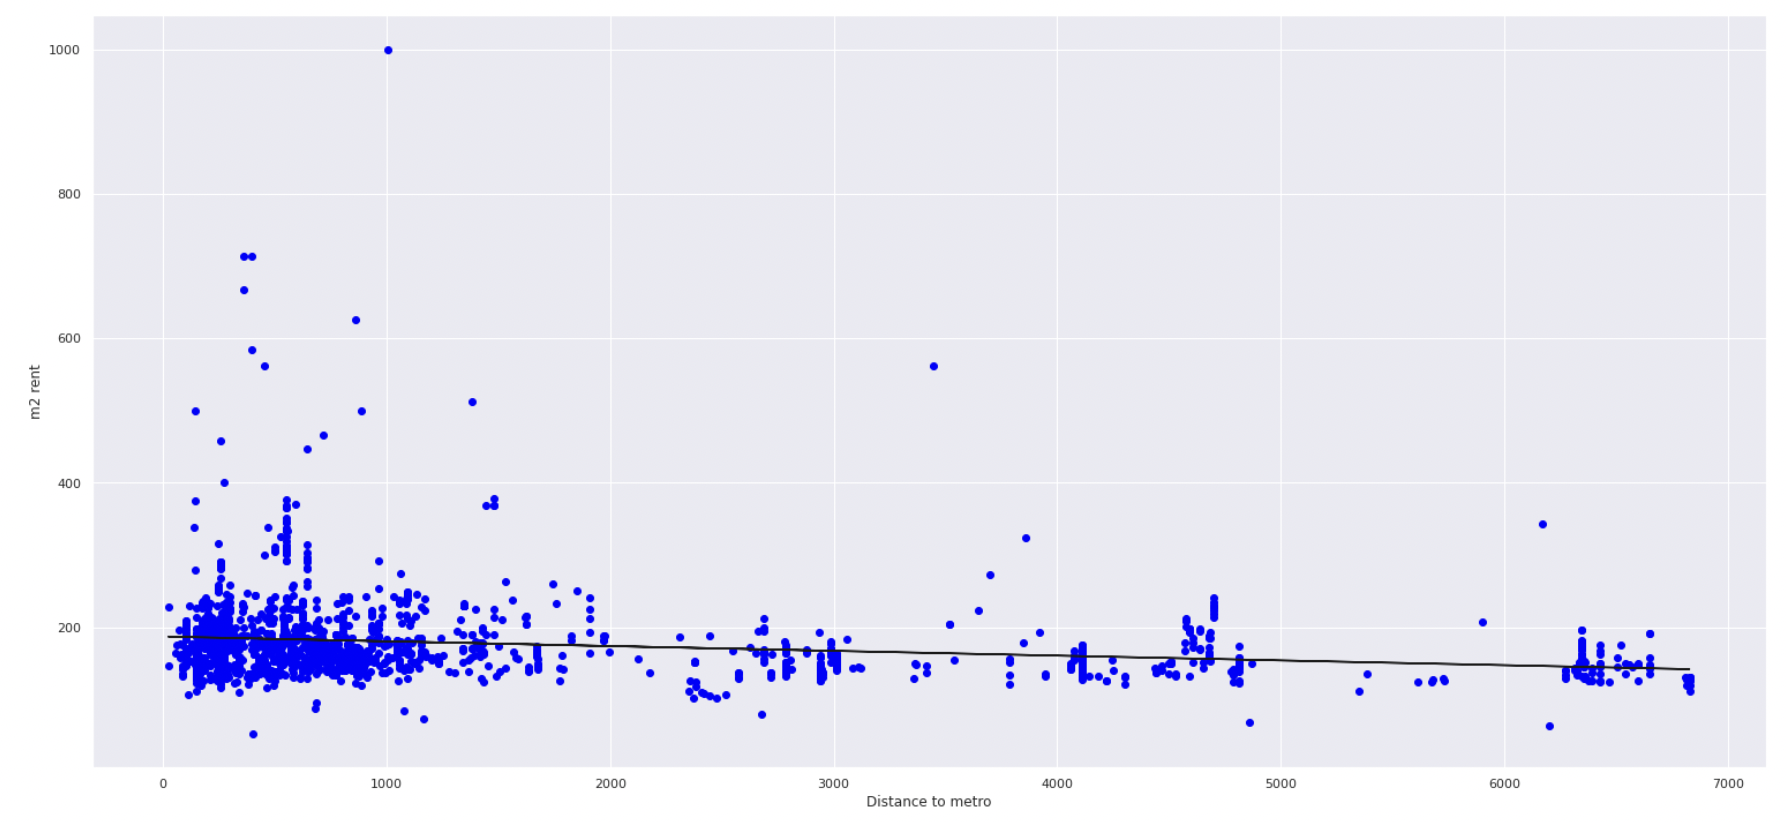
\includegraphics[scale=0.35]{images/LinearReg_boligzonen.png}
    \caption{Distance to metro and normalized rent}
    \label{fig:dist_boligzonen}
\end{figure}



\subsection{Boligsiden}

The results of \textbf{Moran’s I} on the Boligsiden data are provided in table \ref{morans_I_boligsiden} for each choice of \textit{k}-nearest neighbour in the spatial weights. For all \textit{k}-values we see a significant pseudo p-value, i.e. below the standard 0.05, and we can for each case reject the null hypothesis. Appendix B shows the Monte Carlo distributions of randomized data compared to the Moran's I values. As we have done multiple hypothesis tests (4), we may correct the p-value threshold with Bonferroni Correction: $threshold = \frac{\alpha}{n} = \frac{0.05}{4} = 0.0125$. As such, all the tests still pass significance. Furthermore, since the Moran's I value is positive in each case, we can say that apartments with high and/or low rent are spatially clustered more than we would randomly expect. This is again clearest when \textit{k} equals \textit{2}. Generally, the Boligsiden data shows a higher spatial autocorrelation than the data from Boligzonen.

\begin{table}[h]
\renewcommand{\arraystretch}{1.3}
\label{morans_I_boligsiden}
\centering
\begin{tabular}{|c|c|c|c|}
\hline
\bfseries \textit{k-value} & \bfseries Moran's I & \bfseries pseudo p-value\\
\hline\hline
2 & 0.9 & 0.01 \\
6 & 0.85  & 0.01 \\
8 & 0.84 & 0.01 \\
10 & 0.84 & 0.01 \\
\hline
\end{tabular}
\caption{Moran's I results for different values of \textit{k}-nearest neighbor in adaptive kernel spatial weights on the Boligsiden data.}
\end{table}

\begin{figure}[!htbp]
    \centering
    \includegraphics[scale=0.4, trim={0 6cm 0 4cm},clip]{images/cluster_sydhavn.png}
    \caption{Cluster of Boligsiden apartments in Sydhavn}
    \label{fig:cluster_sydhavn}
\end{figure}


The results of \textbf{metro distance and rental price correlation} on Boligsiden data are provided in figure \ref{fig:dist_boligsiden}. Similar to Boligzonen the figure shows that most apartments are within a thousands meter to the nearest metro and that the normalized rental price for these apartments vary a lot even for apartments with the same distance to the metro. Performing the linear regression method we get the result of the R-squared value to be 0.023 and the result of the coefficient to be -0.0108. Only 2,3\% of the variance in the rental price can be explained by the distance to the metro. The coefficient represents the mean decrease in rental price for every additional meter to the nearest metro. If the distance increases by 1 meter, the average rental price decreases by 0.0108 Danish crowns.

\begin{figure}[!htbp]
    \centering
    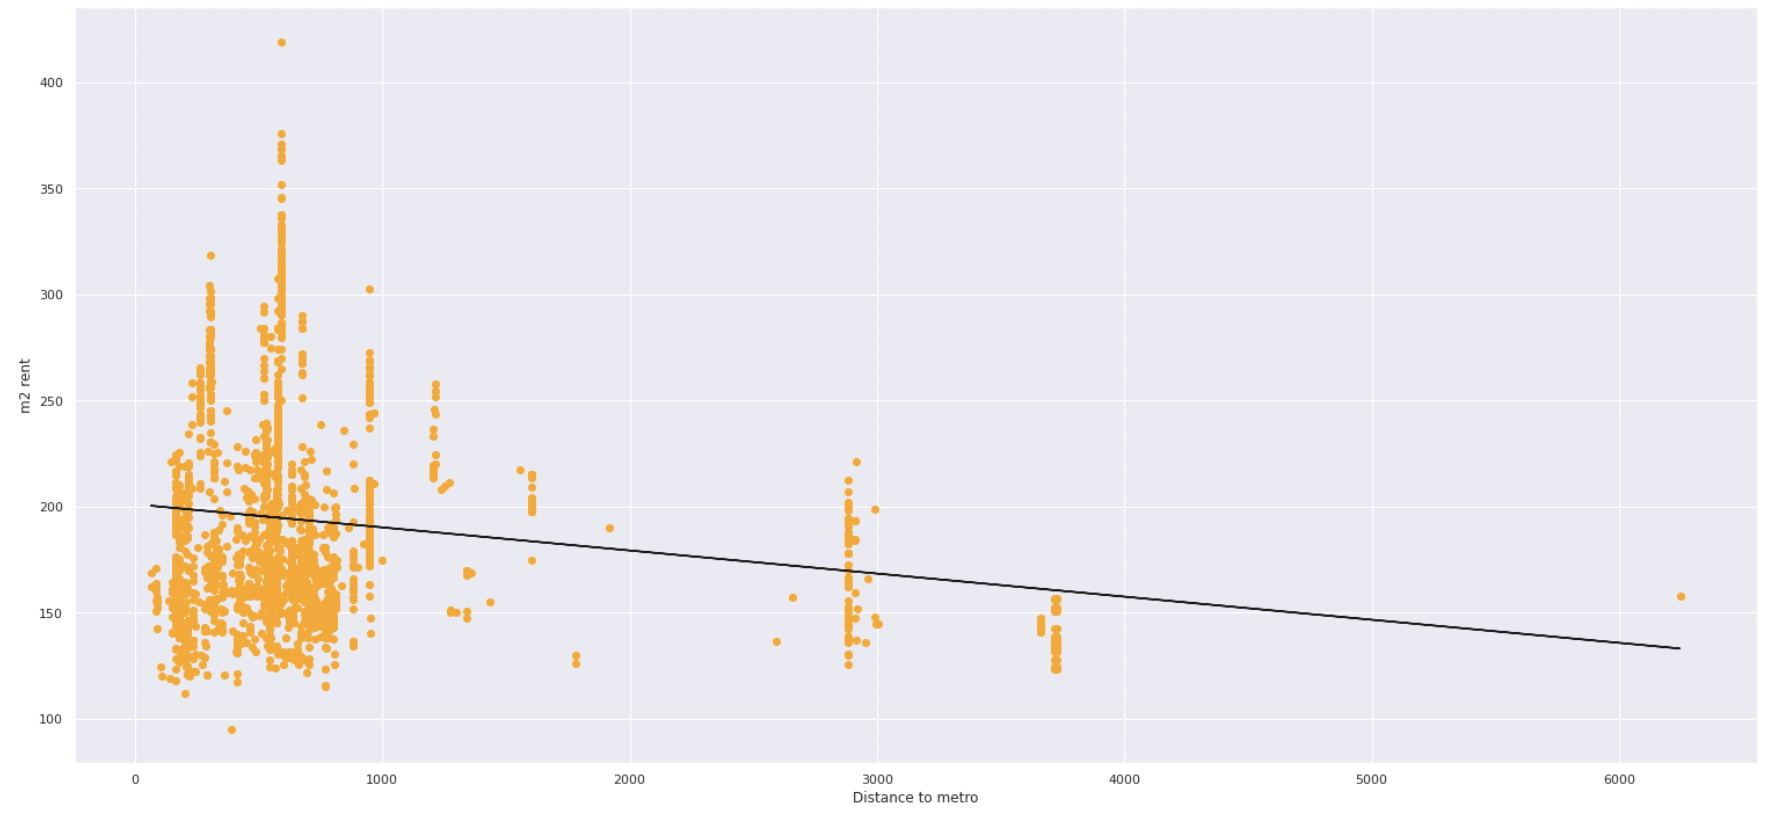
\includegraphics[scale=0.35]{images/LinearReg_boligsiden.png}
    \caption{Boligsiden - Distance to metro and normalized rent}
    \label{fig:dist_boligsiden}
\end{figure}


\subsection{Inverse distance weighted interpolation of Boligzonen rent values}
Boligsiden dataset was not used for interpolation because its apartments are located mainly along the main canal and majority are higly clustered. Boligzonen data was used because of its coverage of city area. Initially interpolated value was price per area but it did not produce satisfying results because there was no underlying pattern to be generalised. It can be observed on the interactive map (kepler.gl) that location has small influence on rent per area price. Rent was better suited as clusters of higher prices can be observed in the central part of Copenhagen as well as in the new buildings in Amager. In figure \ref{fig:interpol} we can see the results of interpolating grid of 50 x 40 points [horizontal x vertical], from 10 nearest neighbours for each point, with power parameter equal to 1.
\begin{figure}[!htbp]
    \centering
    \includegraphics[scale=0.5, trim={0 6cm 0 4cm},clip]{images/rent_D-10_K-10_P-1.png}
    \caption{Interpolated rent values of Boligzonen apartments}
    \label{fig:interpol}
\end{figure}
This interpolation is more valid in places in close proximity to apartments. South-west and west areas of Copenhagen are not representative because of few number of apartments in that area. Values of rent near city boundaries are influenced by edge effect as all apartments used for interpolation lie inside them. Eastern part of Copenhagen is also influenced by natural boundary, Baltic sea, which is not a popular apartment area. In figure \ref{fig:interpol_apart} we can see results of interpolation from figure 6 with added location of apartments for deducing which part of the interpolation is more trustworthy than other.

\begin{figure}[!htbp]
    \centering
    % \includegraphics[scale=0.5]{images/rent_D-10_K-10_P-1.png}
    \includegraphics[scale=0.5, trim={0 6cm 0 4cm},clip]{images/rent_apartments_D-10_K-10_P-1.png}
    \caption{Interpolated rent values of Boligzonen apartments with their location}
    \label{fig:interpol_apart}
\end{figure}


%\medskip
%\begin{tabular}{lrrrrrr}
%\centering
%  \toprule
%  Instance name & $n$ & A & F & M & N & S \\
%  \midrule
%bht.txt                  & 5757    & F   & 0    & ?!   & 6      & T        \\
%common-1-500.txt         & 500     & F   & -1   & ?!   & -1     & F     \\
%common-1-5000.txt        & 5000    & T   & 1    & ?!   & -1     & T     \\
%common-1-5757.txt        & 5757    & T   & 1    & ?!   & -1     & T       \\
%\toprule
%\end{tabular}
%\medskip

% Provide and explain the results of your investigation, illustrated with figures where essential and relevant (unlike figure \ref{fig01}). Relate to lessons learnt, counts, statistics, maps or other outcomes.
% Briefly comment on 1) the main elements of your digital workflow, highlighting challenges and decision-making bottlenecks (e.g. how did you transform point data to make it into a continuous surface?) 2) functions/tricks you found useful and wish to promote or credit. Remember that the technical tasks should not clutter/interfere with your overall narrative and data analysis (unless your project is about developing a technical pipeline) 
% For 'technical pipeline' projects: provide a guided tour of your pipeline to facilitate its reproducibility, explaining your choices, clarifying dependencies, and referring to the scripts/tools you compiled in GitHub.

\section{Discussion}
There were not many ready to use datasets with apartment data, and we didn't manage to find one for Copenhagen. Lot of effort was dedicated to obtaining data and cleaning it. This seems to be a recurring theme in the geo-spatial analysis connected to apartments as we read in \cite{monit}. 

Looking at the results of Moran's I, we see a clear reflection of the underlying method choices in the outcome of the study. For some apartments in the data, the choice of a low \textit{k} defines a neighborhood as within a single building, while for less dense areas the neighborhood is a bit larger. A lower choice of \textit{k}-nearest neighbour in the spatial weights resulted in a higher spatial autocorrelation. It seems obvious that rental prices within single buildings are related in a way that does not necessarily reflect the area around it. Therefore, we suggest that autocorrelation with low \textit{k}'s do not alone paint a picture of rentals price clustering in Copenhagen. On the other hand, the varying density of apartments in Copenhagen, and in the data in particular, does not allow for a single choice of \textit{k}. For that reason, we further suggest that autocorrelation of rental pricing in Copenhagen must be evaluated using multiple values of \textit{k} as each impose a certain structure on the city areas.

The two data sets represent subsets of the rental market in Copenhagen, and we cannot know for sure if the union of both of of them represents Copenhagen as a whole. Both data sets may contain sampling biases as they likely attract certain types of rentals. For example, we know by experience that some apartments are rented out to friends and family without being posted on any platforms. These apartments are not taken into account in the analysis even though they do make up a part of the rental market in Copenhagen. Further, some apartments are solely posted on social platforms, like Facebook, which we have not taken into account. We also know that since it costs money to post an apartment on Boligsiden, the platform is likely to attract commercial renters. This incentives whole apartment blocks in the data, which may explain the higher tendency for spatial autocorrelation in the Boligsiden data. 

Although the coverage of Copenhagen of Boligzonen apartment was much better than of Boligsiden, interpolation results matched apartments rent price only in some areas. This was caused not only because of the imperfect data but also because of the chosen algorithm - inverse distance weighting. Only after seeing that results are worse than expected we found out that IDW is not the best algorithm for such interpolation, \cite{prices}. It causes bulls eye effect which are concentric areas of the same values. Luckily, we did not observe extreme cases of that effect.

Even if the data sets do not represent Copenhagen as a whole, the analysis on them still tells a story; That part of the rental market in Copenhagen is spatially autocorrelated such that apartments with high and/or low rent are spatially clustered more than we would randomly expect. In a broader perspective, it means that there are spatial areas in Copenhagen with similar rent prices.

\subsection{The distance to the metro}
From both Boligsiden and Boligzonen the results showed quite small R-squared values. Hence we might question whether the linear regression can be used to describe the correlation between the distance to the nearest metro and rental price per square meter. Since we are not using the linear regression model for prediction but to explain a correlation, the R-squared value is not as important. Meaning we might conclude that the distance to the metro has a very weak influence on the price. However looking at the figure it might be more correct to say that since most apartments in Copenhagen are close to a metro station there might be some other variables that have a greater impact on the normalized rental price. For example the number of rooms which is illustrated on figure \ref{fig:metro_norm_rent}. 

\begin{figure}[H]
    \centering
    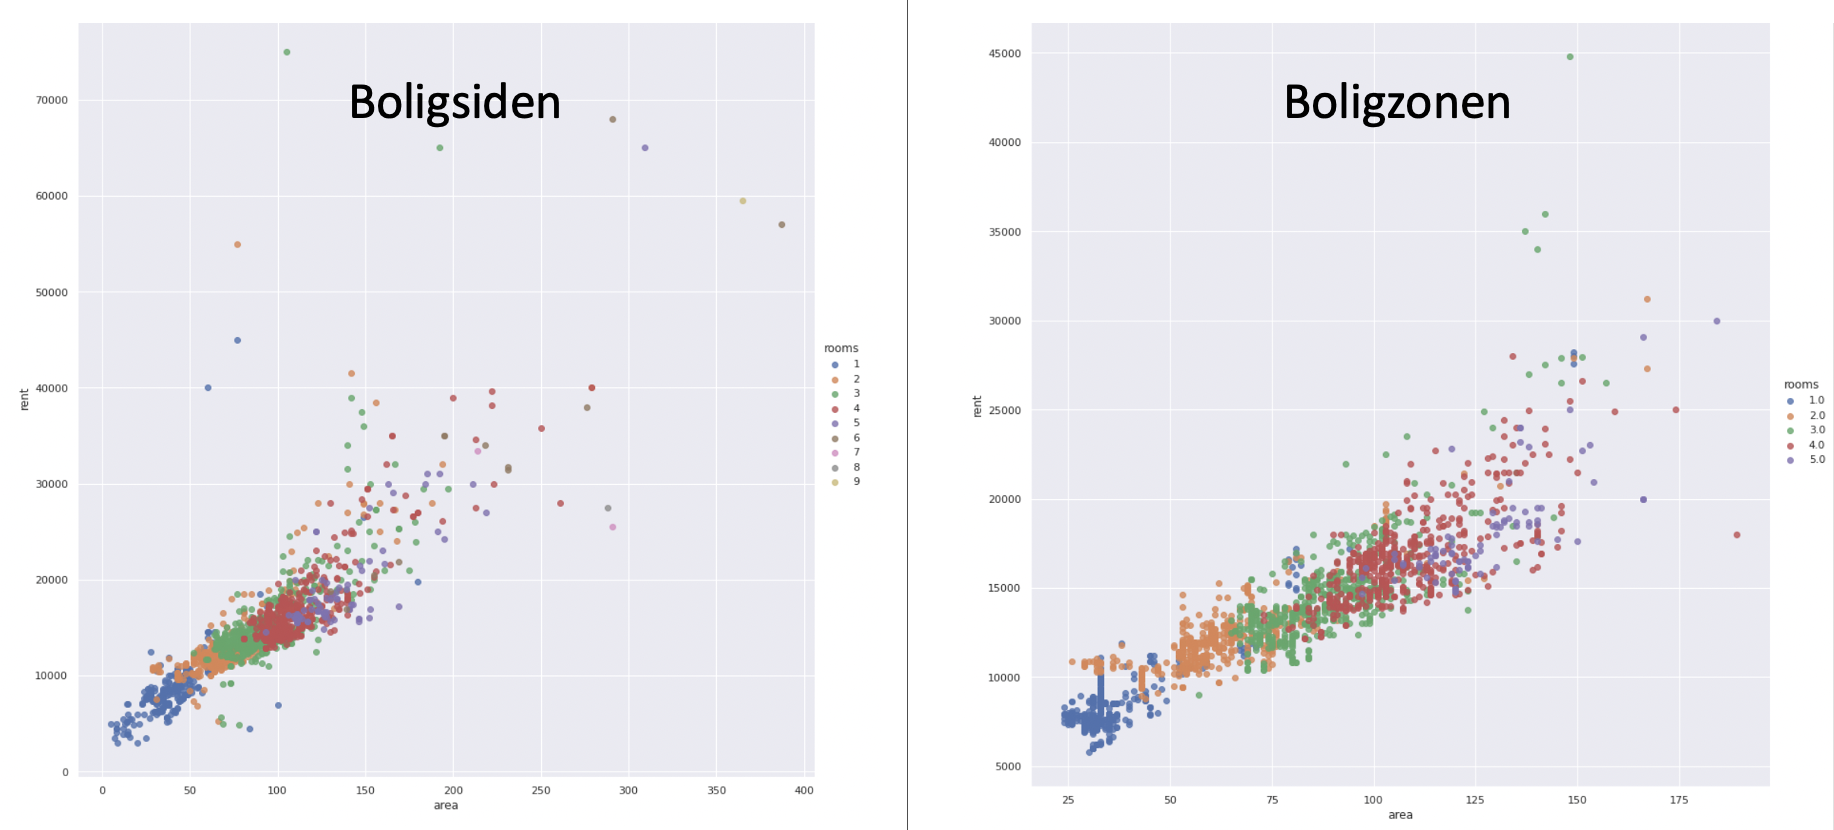
\includegraphics[scale=0.4]{images/room_area_price.png}
    \caption{Boligsiden - Distance to metro and normalized rent}
    \label{fig:metro_norm_rent}
\end{figure}

For a future analysis it might be interesting to look further into location and the distance to the water because this is known to have impact on properties for selling and buying. With more complete data sets it could be interesting to look at energy use, year of construction, balcony, other facilities and the general conditions of the rental place. 


%% Comment on data: What does the analysis on the two datasets represent; Which type of sample of whole Copenhagen?


%Evaluate the results in light of the data sources and research premises/assumptions. How representative, reliable, complete and precise are your results? How transferable or generalizable? Give an account on the major short-coming(s) of your methodology / data / prototype. Briefly evaluate the results in light of digital tools, the learning process, time on task, vis-à-vis the final product.

\section{Conclusion}
% Here you provide a short summary of the results of the project, the achieved (or missed) goals and highlight the most important lessons learnt while working on the project. Indicate how the methods, data, analysis, or prototype functionalities could be improved or extended in future work.

Overall we can conclude that location influences the rent in Copenhagen in the sense that the rental market is spatially autocorrelated. Rental apartments with low rent are more likely to be clustered in the same way that rental apartments with high rent are more likely to be clustered. The reason for this could be that the data sets contains a large amount of project apartments or apartment blocks where one landlord is renting out multiple apartments. \\
Furthermore we reach the conclusion that there is a weak correlation between the distance to the metro and the rent. The reason being that most apartments within Copenhagen centre is fairly close to a metro and therefore are more influenced by some other variables. For example we see a stronger correlation between the number of rooms and rent. 

\bibliography{references}

\section*{Appendices}

\subsection{Appendix A}
\label{appendix_a}

Figure \ref{boligzonen_k_2}, \ref{boligzonen_k_6}, \ref{boligzonen_k_8} and \ref{boligzonen_k_10} show Monte Carlo distributions and Moran Scatterplot for \textit{k}-values of 2, 6, 8 and 10, respectively, for Boligzonen data. Each Moran's I value lies outside of the Monte Carlo distribution.

\begin{figure}[H]
    \centering
    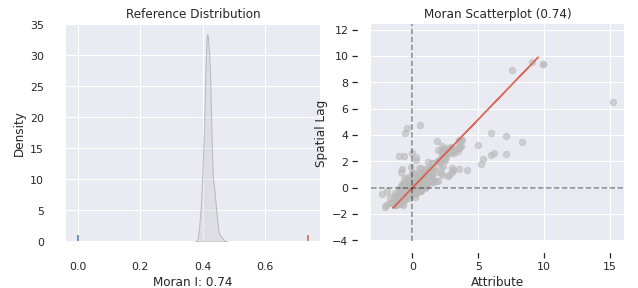
\includegraphics[width=1\textwidth]{images/morans_i_k_2.png}
    \caption{Moran's I plot for Boligzonen of k=2.}
    \label{boligzonen_k_2}
\end{figure}

\begin{figure}[H]
    \centering
    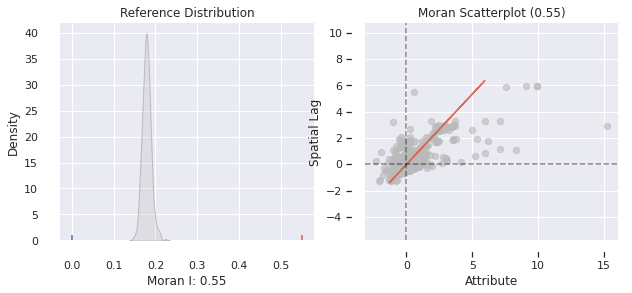
\includegraphics[width=1\textwidth]{images/morans_i_k_6.png}
    \caption{Moran's I plot for Boligzonen of k=6.}
    \label{boligzonen_k_6}
\end{figure}

\begin{figure}[H]
    \centering
    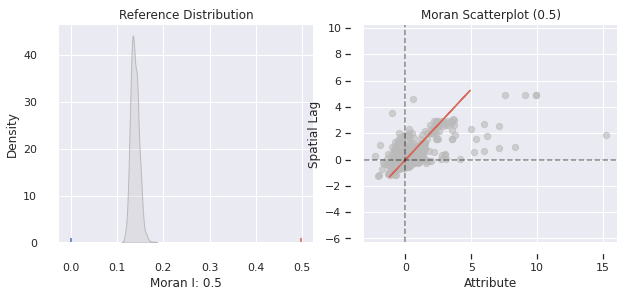
\includegraphics[width=1\textwidth]{images/morans_i_k_8.png}
    \caption{Moran's I plot for Boligzonen of k=8.}
    \label{boligzonen_k_8}
\end{figure}

\begin{figure}[H]
    \centering
    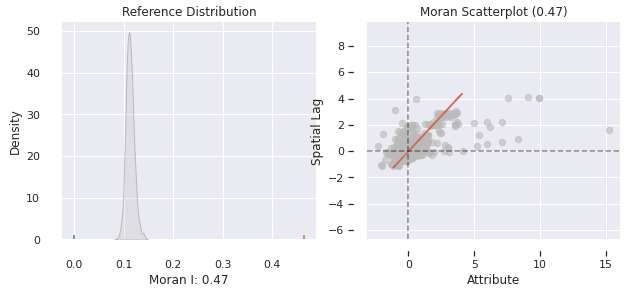
\includegraphics[width=1\textwidth]{images/morans_i_k_10.png}
    \caption{Moran's I plot for Boligzonen of k=10.}
    \label{boligzonen_k_10}
\end{figure}

%Metadata tables – see project report for details

\section*{Appendix B: Contribution statement}

% For individualized grading, you must provide a contribution statement in which you clarify who of your group is responsible for the different parts of the project submission. Please state:

% \begin{itemize}
%     \item For \textbf{at least 2 sections} of your report, who was \textbf{primary contributor} (and optionally also second and/or third contributor)
%     \item For any \textbf{additional major tasks} such as data collection, data preparation, analysis, programming, or visualization, who was \textbf{primary contributor} (optionally also second and/or third contributor)  
% \end{itemize}
\textbf{Szymon} : Python scraper for Boligzonen, Go scraper for Boligzonen, Eliminating duplicates, Interactive map in Kepler.gl, IDW interpolation, Visualisation in general,
Sections: 2.2, 3.2, 3.3, 4.5, 5.3

\end{document}